\section{Motivation} \label{sec:motivation}

In this section, we discuss two weaknesses in the state-of-the-art function merging optimization~\cite{rocha20}.
First, we show that there is a significant opportunity in reduction that can be gained by having a better profitability analysis.
%Second, we show that we can save compilation time by bailing out early from unprofitable merge operations, avoiding wasteful merges.
Second, we show that most function merging attempts are trown away as they cause code bloat, according to the profitability analysis.

\subsection{Inaccuracies in the Profitability Analysis}

Although the proposed technique is able to merge any two functions, it is not always profitable to do so.
A pair of functions can be profitably merged when replacing them by the merged function results in an overall smaller code.
As it is only profitable to merge functions that are sufficiently similar, for most pairs of functions, merging them increases code size.
Since the profitability analysis is critical for the optimisation strategy, we must be able to effectively decide which pair of functions can be profitably merged.

In order to estimate the code-size benefit, we first estimate the size of all three functions, i.e., the two input functions and the merged one.
The size of each function is estimated by summing up the estimated binary size of all instruction in the function, in its IR form.
The binary size of each IR instruction is estimated by querying the compiler's built-in target-specific cost model.
These cost models provide target-dependent cost estimations approximating the code-size cost of an IR instruction when lowered to machine instructions.

As pointed out by many prior work~\cite{porpodas18,rocha19,rocha20}, even though cost models offer a good trade-off between compilation time and accuracy, they are expected to contain inaccuracies.
Because we are trying to estimate the binary size of the final object code, inaccuracies arise from the fact that we are operating on the IR level and one IR instruction does not necessarily translate to one machine instruction.
Because we are operating on the IR level, We cannot know exactly how each IR instruction will be lowered without actually running the compiler's backend.
Moreover, several number of optimisations and code transformations will still run prior to machine code generation.
%The same IR instruction can be lowered to different machine instructions, depending on its surrounding context, the instruction selection algorithm, and many other factors.
%Therefore, there is also an inherent limitation of estimating the cost of each instruction separately of its context.

Figure~\ref{fig:oracle-reduction} presents the code size reduction that can be achieved with an oracle.
This oracle measures code size by compiling the whole program down to its final object file, which provides perfect information for the cost model.
It shows the potential for improvement there exists from having a better profitability analysis, almost doubling the reduction.
By compiling the whole program down to its binary form, we are able to precisely capture the impact on other optimizations and machine code generation, as well as the overheads that result from replacing the callsites to the merged function or keeping a \textit{thunk}.

\begin{figure}[h]
  \centering
  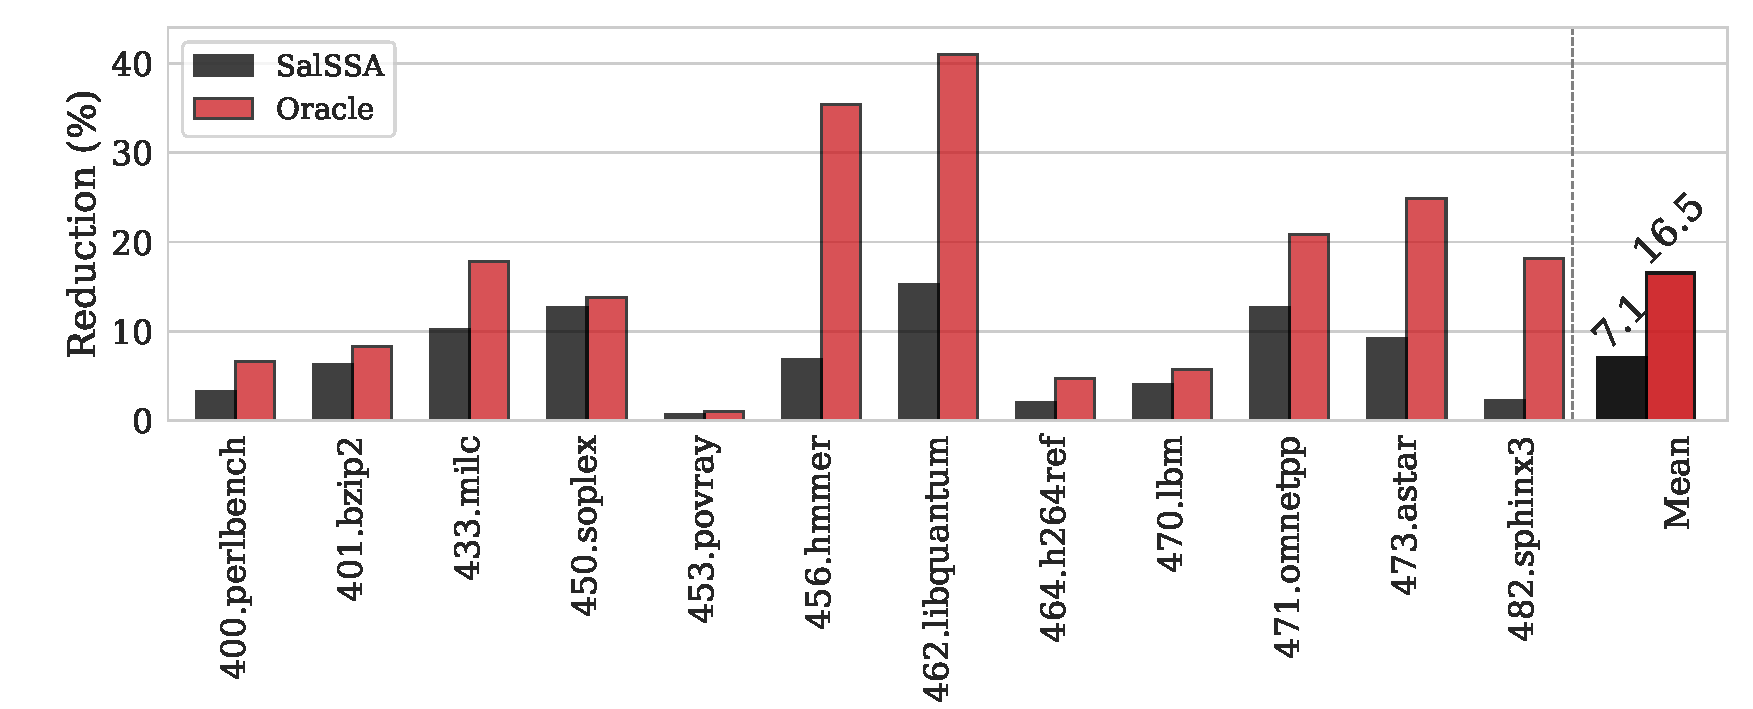
\includegraphics[width=0.5\textwidth]{figs/motivation-oracle-reduction.pdf}
  \vspace{-2.5em}
  \caption{.}
  \label{fig:oracle-reduction}
\end{figure}

However, the cost of compiling the whole program for every merging attempt is prohibitive.
The re-compilation overhead can be severely aggravated for larger programs with multiple functions, where not only each compilation takes longer but the whole program is also re-compiled many times.

\subsection{Wasteful Merge Operations}

The fingerprint-based ranking strategy helps the function merging optimization to pair functions that are more similar.
However, the current strategy is unable to decide which one of those pairs are actually worth merging.
Figure~\ref{fig:unprofitable-attempts} shows that about 82\% of the top ranked candidate functions are actually unprofitably merged.
As a result, a considerable amount of compilation time is wasted producing merged functions that will be thrown away, keeping the original pair of functions.

\begin{figure}[h]
  \centering
  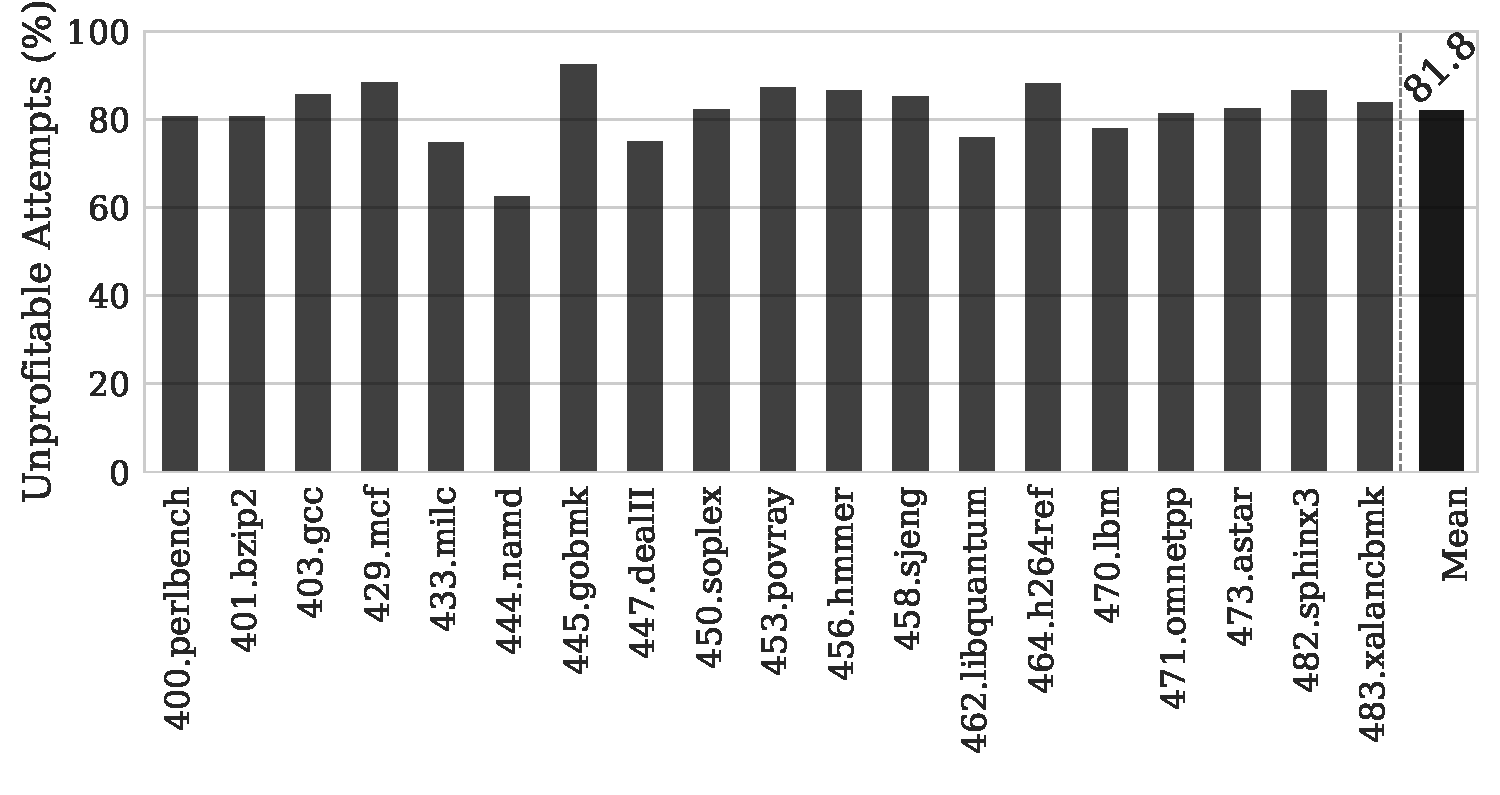
\includegraphics[width=0.5\textwidth]{figs/unprofitable-attempts.pdf}
  \vspace{-2.5em}
  \caption{An average of about 82\% of merging attempts are unprofitable.}
  \label{fig:unprofitable-attempts}
\end{figure}

%Figure~\ref{fig:compilation-breakdown} shows a breakdown of the time spent in different steps of the function merging optimization.
%As expected, this breakdown confirms that most of the compilation-time is spent merging functions, which includes both the sequence alignment and code generation.
%This also includes the time wasted producing unprofitable merged functions.
%Therefore, it is important to avoid merging unprofitable functions.

Figure~\ref{fig:unprofitable-compile-time-percentage} shows the time spent producing unprofitable merged functions relative to the total compilation time of the function merging optimization.
Since most of the merged functions are thrown away for being unprofitable, it is expected that most of the compilation time is also spent producing those merged functions.
However, this impact is also aggravated when several of the unprofitable merged functions are much larger than the profitable ones.

\begin{figure}[h]
  \centering
  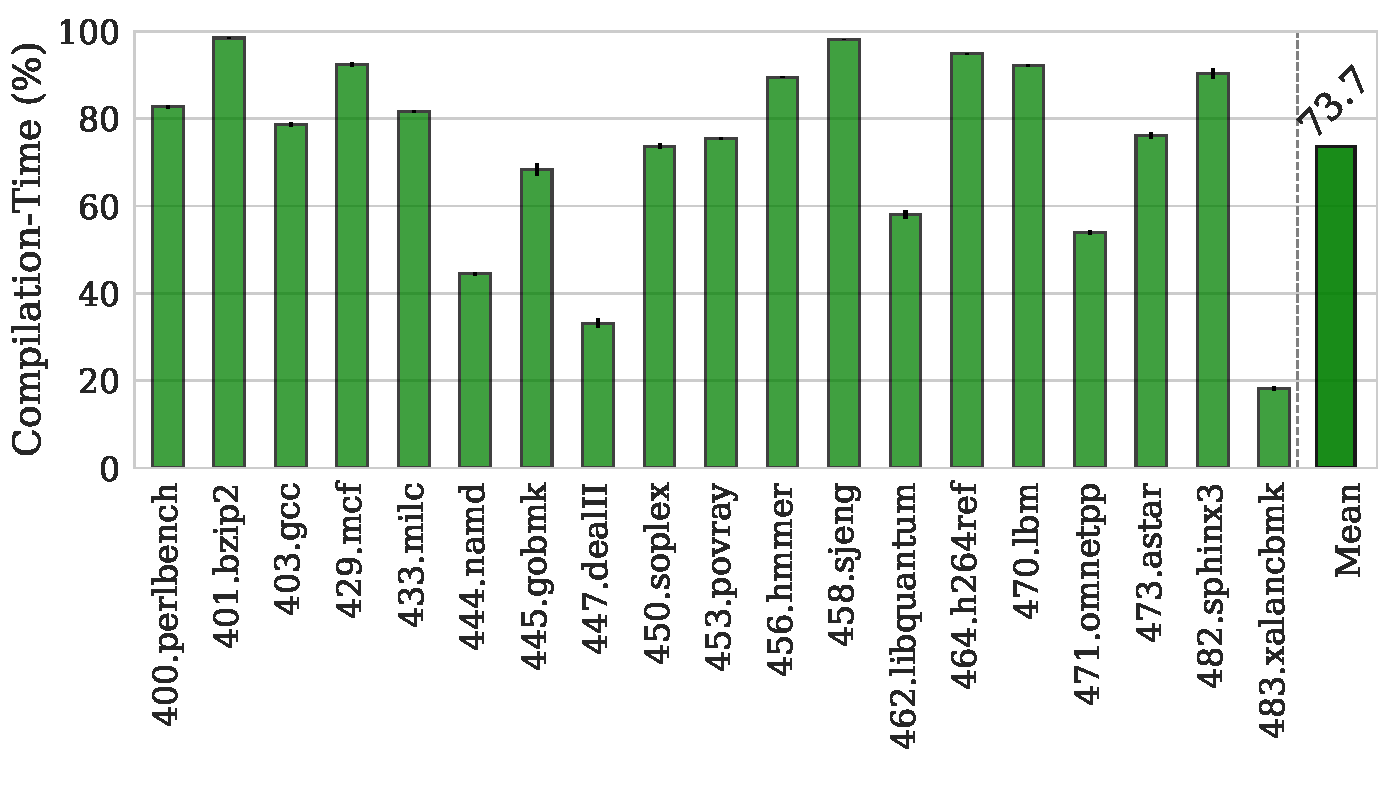
\includegraphics[width=0.5\textwidth]{figs/unprofitable-compile-time-percentage.pdf}
  \vspace{-2.5em}
  \caption{The percentage of compilation-time spent on unprofitable merge operations.}
  \label{fig:unprofitable-compile-time-percentage}
\end{figure}

Therefore, it is of utmost importance that we avoid merging unprofitable functions.
If we could eliminate all the time wasted on unprofitable merge operations, we would free compilation time for more useful computation.

\subsection{Summary}

In this paper, our goal is to develop a solution capable of identifying whether or not a given pair of functions can be profitably merged, allowing us to use a more expensive profitability analysis based on partial re-compilation.
If we could predict which pairs of function are more likely to cause code bloat, we could avoid wasting time merging them in the first place and having to estimate their binary sizes.
Bailing out early frees time to be spent on more profitable merge operations.


